Consider the 30 observations on male Egyptian skulls for the first time period given in Table 6.13 on page 349.

\begin{enumerate}[label= (\alph*)]
    \item Construct \textit{Q-Q} plots of the marginal distributions of the maxbreath, basheight,
    baslength and nasheight variables. Also, construct a chi-square plot of the
    multivariate observations. Do these data appear to be normally distributed?
    Explain.

    \begin{figure}[H]
        \centering
        \begin{tabular}{cc}
            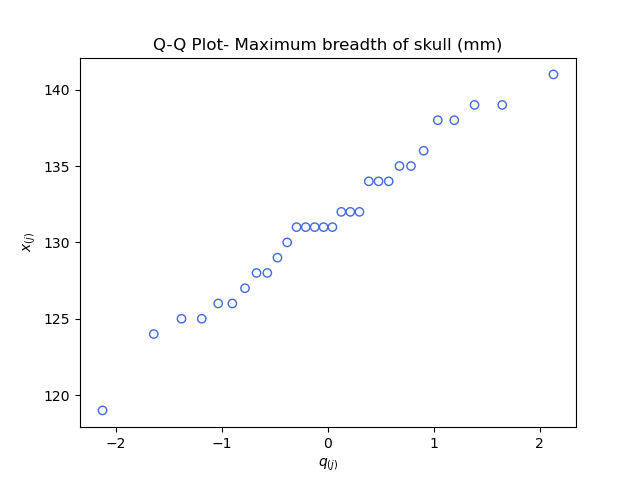
\includegraphics[scale=0.30]{./python/chapter-5/Question-5-23-a-QQ-MaxBreath.png} &
            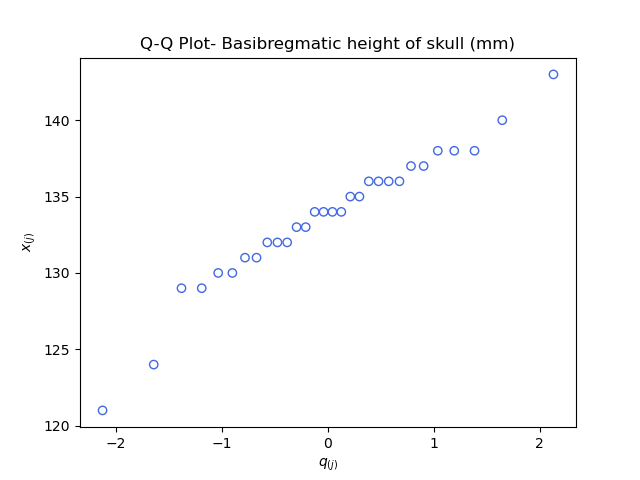
\includegraphics[scale=0.30]{./python/chapter-5/Question-5-23-a-QQ-BasHeight.png} \\
            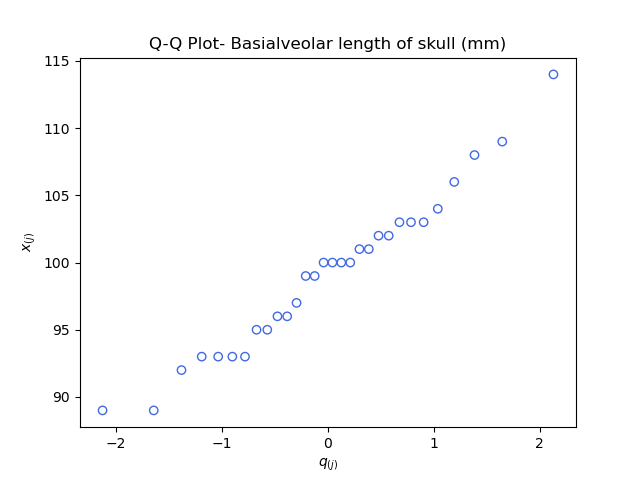
\includegraphics[scale=0.30]{./python/chapter-5/Question-5-23-a-QQ-BasLength.png} &
            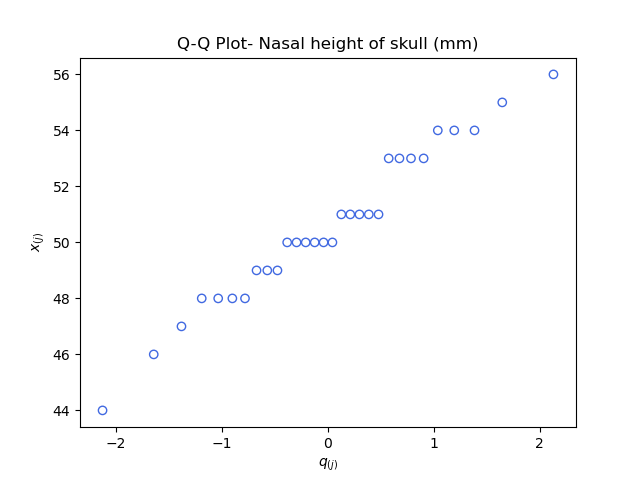
\includegraphics[scale=0.30]{./python/chapter-5/Question-5-23-a-QQ-NasHeight.png}
        \end{tabular}
    \end{figure}

    \begin{figure}[H]
        \centering
        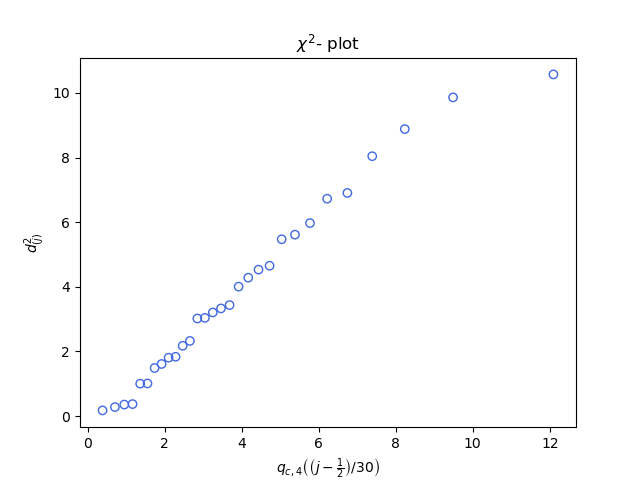
\includegraphics[scale=0.70]{./python/chapter-5/Question-5-23-a-chi2.png}
    \end{figure}

    The \textit{Q-Q} plots look okay. The MaxBreath plot looks really good. There may be a outlier ssmall value though. The plot for BasHeight is very linear, but there are two smaller values out of step. The BasLength plot has observations on either tail, a bit out. The plot for nasal height looks super good. The $\chi^{2}$-plot is alright with a possible outlier or two.

    \item Construct 95\% Bonferroni intervals for the individual skull dimension variables.
    Also, find the 95\% $T^{2}$-intervals. Compare the two sets of intervals.

    \[
        \bar{\textbf{x}}
        =
        \begin{bNiceArray}{r}
            131.367 \\
            133.600 \\
             99.167 \\
             50.533
        \end{bNiceArray}
        \hspace{0.20cm}
        \text{and}
        \hspace{0.20cm}
        \begin{bNiceArray}{rrrr}
            26.309 &  4.152 &  0.454 &  7.246 \\
             4.152 & 19.972 & -0.793 &  0.393 \\
             0.454 & -0.793 & 34.626 & -1.920 \\
             7.246 &  0.393 & -1.920 &  7.637
        \end{bNiceArray}
    \]
    The 95\% $T^{2}$ simultaneous confidence intervals:
    \[
    \bar{x}_{i}
    \pm
    \sqrt{
        \frac{(n-1)p}{(n-p)}
        F_{p, n-p}\left(\alpha\right)
    }
    \sqrt{
        \frac{s_{ii}}{n}
    }
    \]

    \[
        \begin{NiceArray}{rrrr}
        131.37 \pm \sqrt{12.24} \frac{\sqrt{26.31}}{\sqrt{30}} & \text{contains } \mu_{1} & \text{ or } & 128.09 \leq \mu_{1} \leq 134.64 \\
        133.60 \pm \sqrt{12.24} \frac{\sqrt{19.97}}{\sqrt{30}} & \text{contains } \mu_{2} & \text{ or } & 130.75 \leq \mu_{2} \leq 136.45 \\
        99.17 \pm \sqrt{12.24} \frac{\sqrt{34.63}}{\sqrt{30}} & \text{contains } \mu_{2} & \text{ or } & 95.41 \leq \mu_{3} \leq 102.92 \\
        50.53 \pm \sqrt{12.24} \frac{\sqrt{7.64}}{\sqrt{30}} & \text{contains } \mu_{2} & \text{ or } & 48.77 \leq \mu_{3} \leq 52.30
        \end{NiceArray}
    \]
    The 95\% Bonferroni confidence intervals:
\[
    \bar{x}_{i}
    \pm
    t_{n-1}
    \left(\frac{\alpha}{2m}\right)
    \sqrt{
        \frac{
                s_{ii}
            }{
                n
            }
        }
\]

\[
    \begin{NiceArray}{rrrr}
       131.37 \pm 2.66 \frac{\sqrt{26.31}}{\sqrt{30}} & \text{contains } \mu_{1} & \text{ or } & 128.87 \leq \mu_{1} \leq 133.86 \\
       133.60 \pm 2.66 \frac{\sqrt{19.97}}{\sqrt{30}} & \text{contains } \mu_{2} & \text{ or } & 131.43 \leq \mu_{2} \leq 135.77 \\
       99.17 \pm 2.66 \frac{\sqrt{34.63}}{\sqrt{30}} & \text{contains } \mu_{2} & \text{ or } & 96.31 \leq \mu_{3} \leq 102.03 \\
       50.53 \pm 2.66 \frac{\sqrt{7.64}}{\sqrt{30}} & \text{contains } \mu_{2} & \text{ or } & 49.19 \leq \mu_{3} \leq 51.88
    \end{NiceArray}
\]

Dividing the length of the Bonferroni interval by the length of the $T^{2}$ interval,
\[
    \frac{\text{Length of Bonferroni interval}}{\text{Length of the }T^{2}\text{-interval}}
    =
    \frac{t_{n-1}(\frac{\alpha}{2m})}{\sqrt{\frac{(n-1)p}{n-p}F_{p, n-p}(\alpha)}}
    =
    0.7613
\]
The Bonferroni interval is only 76.13\% of the length of the simultaneous $T^{2}$ interval, so it's about 20\% shorter.
    
\end{enumerate}